\chapter{Tribal NeuroSim: kísérleti futtatások és eredmények}

\section{Világ-mechanikák}

A szimuláció terét egy hexagonális rács alkotja. A flexset adatkészletből inicializált futtatások $\approx$36\,100 tile-os térképen játszódnak; a soloq futtatások kisebb világokat kapnak. Minden tile-hoz egy biom-típus van rendelve (DenseForest, Riverland, DrySteppe, Mountains, Marsh, Cold), amely meghatározza az alap élelmiszertermelési rátát.

A törzsek öt polity-szinten fejlődhetnek: \textit{Tribe}, \textit{City}, \textit{Duchy}, \textit{Kingdom} és \textit{Empire}. Minden szintlépéshez populáció-, terület- és szövetségesi küszöbértékek teljesítése szükséges; magasabb szinten több maximális populáció és jobb harci hatékonyság érhető el, de nagyobb élelmiszer-fenntartási igény is keletkezik. Az Empire-szint elérése a győzelmi feltétel: mind a négy teljes futtatás, mind a 103-seed futtatássorozat minden futtatása Empire-szintű győzelemmel zárult.

A harci kimenet Poisson-folyamaton alapul: a várható veszteséget a támadó harci artifactja és a kontaktzóna (a két terület határán szomszédos tile-párok száma) határozzák meg ($\lambda = a_{\text{combat}} \cdot n_{\text{kontakt}} \cdot 0{,}02$), de a konkrét tick-szintű kimenet véletlenszerű. A \textit{liveness-fix} (2026. május 14.) három numerikus hiba javítása volt (a törzs-statisztikák kétszeres normalizálása, a migráció-hajtóerő oszcillációja és a túl konzervatív terjeszkedési küszöb), amelyek korábban statikussá tették a szimulációt. Ettől elkülönül a determinizmus-hiba javítása: a klaszterek rendezetlen SQLite-betöltése különböző tick-sorrenden át különböző kimenethez vezetett, a \textit{clusters.sort\_by(id)} bevezetése után pedig az újrafuttatások bit-azonos eredményt adnak. A részletes fejlődési feltételek és az iteratív tervezési döntések a kibővített verzióban találhatók \cite{premadegraph-full}.

\section{A négy futtatás összefoglalója}

A négy teljes kísérleti futtatás összefoglalója:

Az \ref{tab:neurosim-run-comparison-final} táblázat a négy kísérleti futtatás főbb paramétereit és eredményeit foglalja össze.

\begin{table}[h]
\centering
\small
\caption{A négy záró Tribal NeuroSim futtatás összehasonlítása}
\label{tab:neurosim-run-comparison-final}
\resizebox{\textwidth}{!}{%
\begin{tabular}{|l|l|l|l|l|l|l|l|}
\hline
\textbf{Futtatás} & \textbf{Adatkészlet} & \textbf{Seed} & \textbf{Győztes} & \textbf{Viselkedés} & \textbf{Agresszió} & \textbf{Migráció} & \textbf{Végső tick} \\
\hline
run67fl7777 & Flexset & 7777 & Tribe 355 & Warband/Combat & 0{,}18 & 0{,}88 & 2538 \\
run67fl42 & Flexset & 42 & Tribe 596 & Warband/Combat & 0{,}13 & 0{,}87 & 2487 \\
run67sq42 & SoloQ & 42 & Tribe 89 & Vanguard/Risk & 0{,}11 & 0{,}16 & 2046 \\
run67sq7777 & SoloQ & 7777 & Tribe 70 & Supply/Resource & 0{,}68 & 0{,}87 & 2541 \\
\hline
\end{tabular}
}
\end{table}

A \ref{fig:run-flexset-7777} ábra a flexset seed=7777 futtatásának végállapotát mutatja.

\begin{figure}[H]
\centering
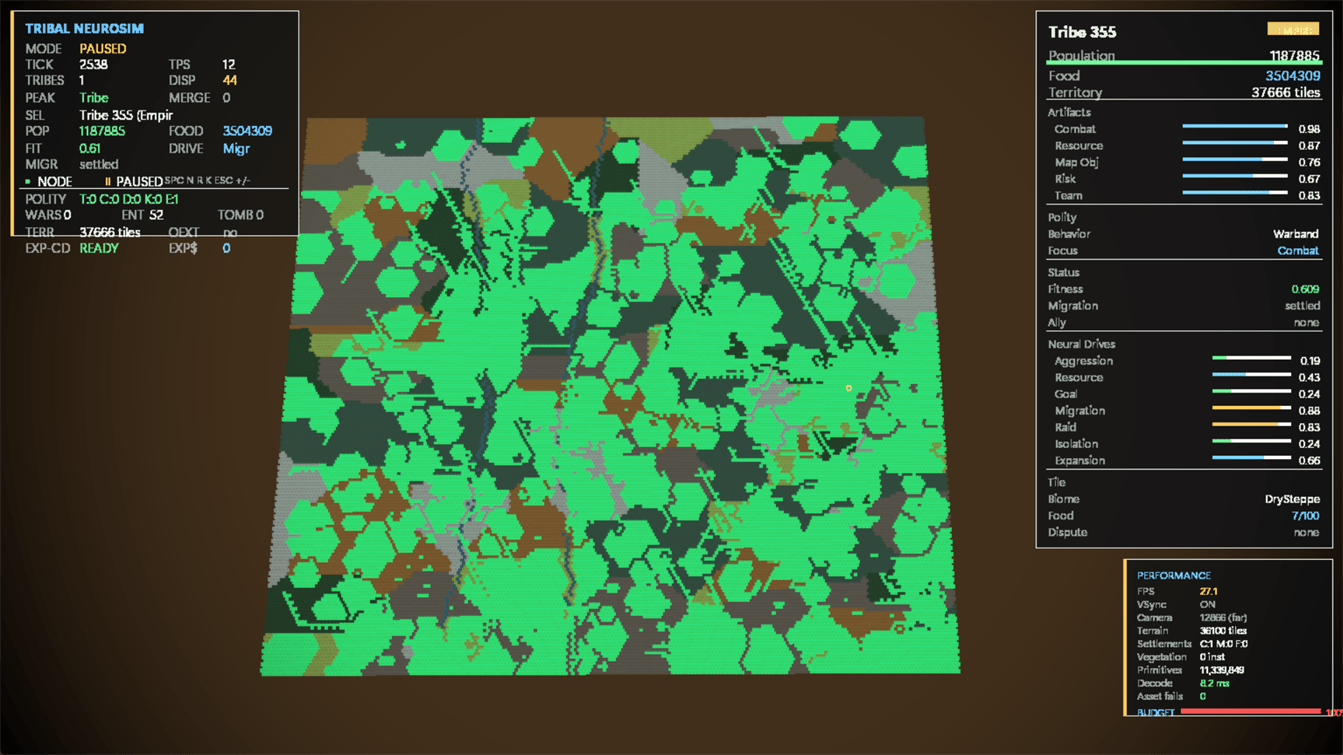
\includegraphics[width=\textwidth]{assets/neurosim/run67fl7777-fl-s7777-tick2538-last.png}
\caption{Flexset, seed=7777, tick=2538: Tribe 355 (Warband/Combat) győzelme, 37\,666 tile-os végső területtel.}
\label{fig:run-flexset-7777}
\end{figure}

A \ref{fig:run-soloq-42} ábra a soloq seed=42 futtatásának végállapotát mutatja, ahol Vanguard/Risk profilú törzs nyert.

\begin{figure}[H]
\centering
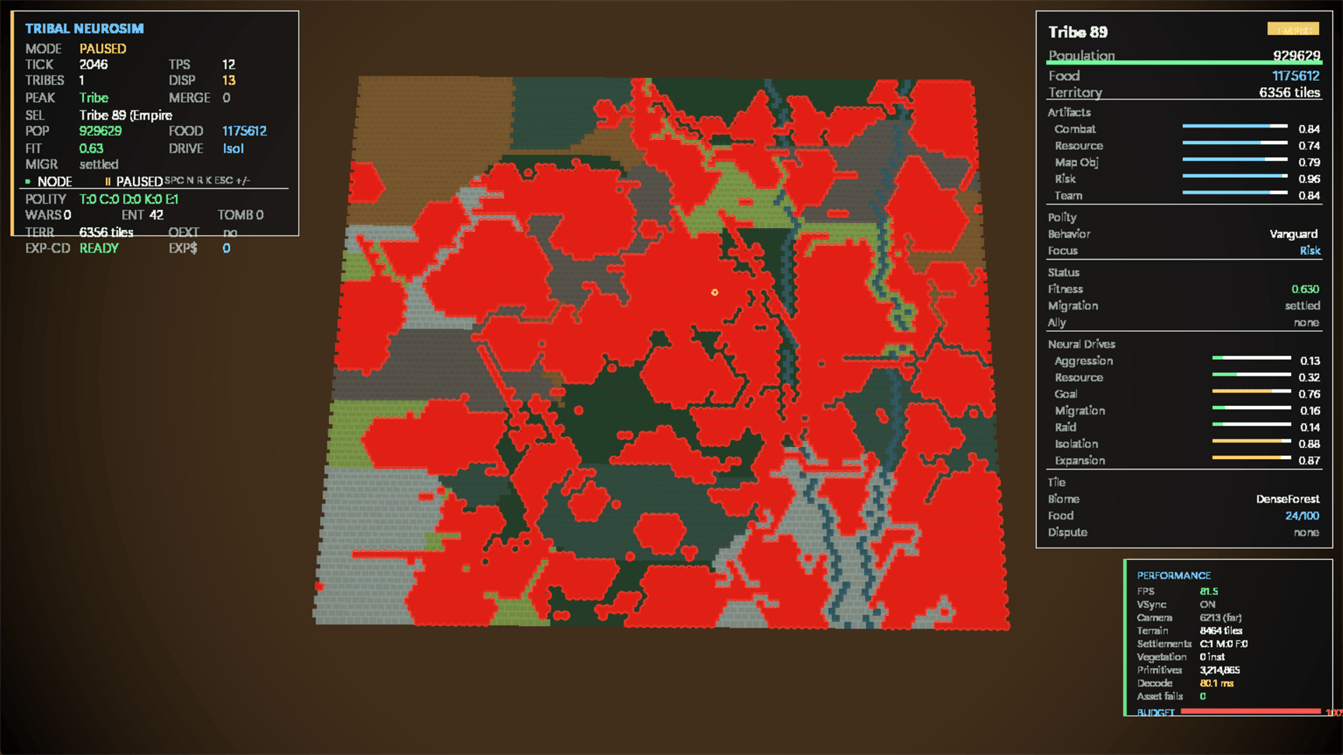
\includegraphics[width=\textwidth]{assets/neurosim/run67sq42-sq-s42-tick2046-last.png}
\caption{SoloQ, seed=42, tick=2046: Tribe 89 (Vanguard/Risk) győzelme, 6\,356 tile-os végső területtel.}
\label{fig:run-soloq-42}
\end{figure}

A \ref{fig:run-soloq-7777} ábra a soloq seed=7777 futtatásának végállapotát mutatja, ahol Supply/Resource profilú törzs nyert.

\begin{figure}[H]
\centering
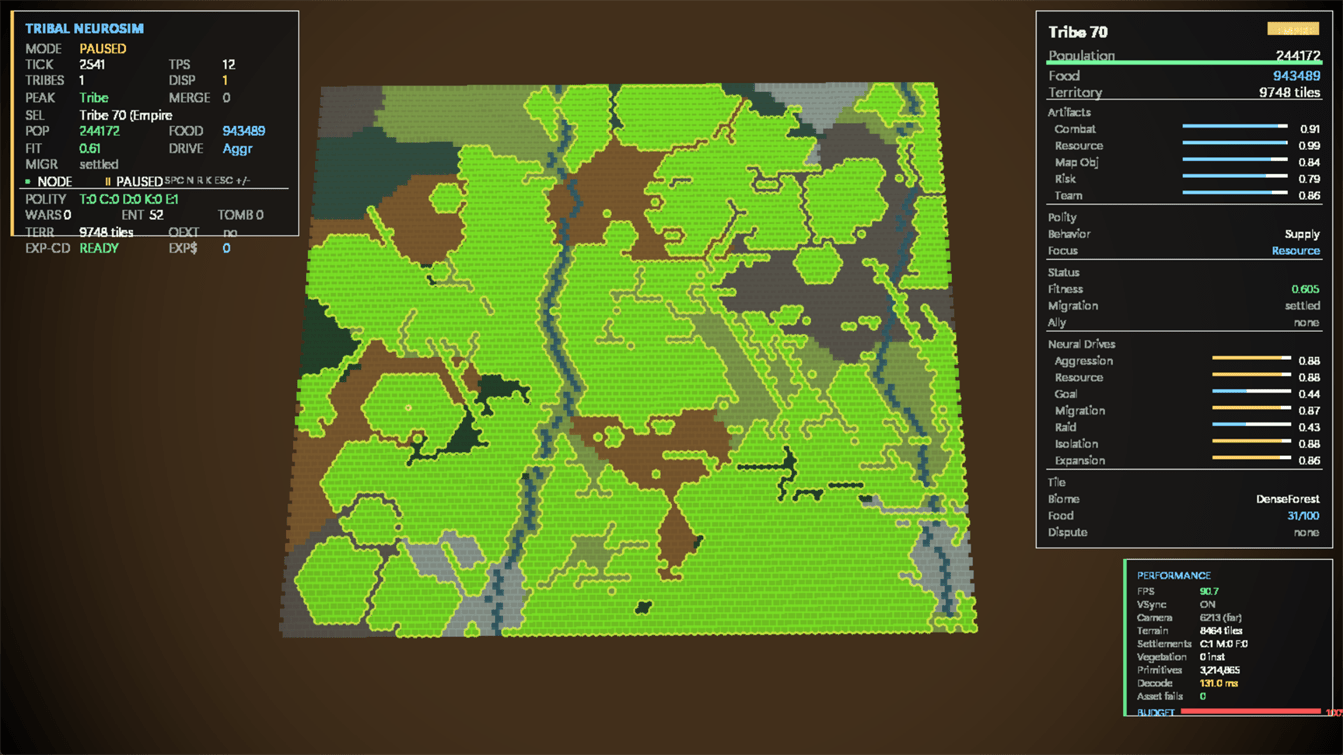
\includegraphics[width=\textwidth]{assets/neurosim/run67sq7777-sq-s7777-tick2541-last.png}
\caption{SoloQ, seed=7777, tick=2541: Tribe 70 (Supply/Resource) győzelme, 9\,748 tile-os végső területtel.}
\label{fig:run-soloq-7777}
\end{figure}

\section{103-seed futtatássorozat és győztes archetípus-eloszlás}

A négy kísérleti futtatást egy 103-seed soloq futtatássorozat egészíti ki. Minden futtatás Empire-szintű győzelemmel zárult (103/103). Az archetípus-eloszlás:

Az \ref{tab:soloq-sweep-archetypes} táblázat a 103-seed soloq futtatássorozat győztes archetípus-eloszlását tartalmazza.

\begin{table}[H]
\centering
\caption{Győztes archetípus-eloszlás a soloq 103-seed futtatássorozat alapján}
\label{tab:soloq-sweep-archetypes}
\begin{tabular}{|l|r|r|}
\hline
\textbf{Archetípus} & \textbf{Futtatások} & \textbf{Arány} \\
\hline
Warband   & 36 & 35{,}0\% \\
Supply    & 23 & 22{,}3\% \\
Council   & 20 & 19{,}4\% \\
Vanguard  & 14 & 13{,}6\% \\
Pathfinders & 10 & 9{,}7\% \\
\hline
\textbf{Összesen} & 103 & 100\% \\
\hline
\end{tabular}
\end{table}

Az átlagos befejezési tick 2308{,}57; az átlagos győztes terület 8\,338 tile. A Warband archetípus enyhe pluralitással vezet (35\%), de nem rendelkezik erős, seed-független dominanciával.

A 103-seed futtatássorozat naplóállományai futtatásonként közel 35\,000 soros JSONL-formátumú eseménynaplót tartalmaznak. A keletkező adatmennyiség összesítéséhez és az archetípus-eloszlás azonosításához mesterséges intelligencia alapú szövegelemző eszközt alkalmaztunk; az összesített statisztikákat ezt követően manuálisan ellenőriztük.

\section{Mit mutatnak az eredmények}

A két tesztelt flexset futtatás (seed=42 és seed=7777) mindkét esetben Warband/Combat profilú entitás győzelmével zárult, alacsony agresszióval (0{,}13–0{,}18) és magas migrációval (0{,}87–0{,}88). A soloq futtatások változékonyabb győztesprofilt produkáltak: seed=42 Vanguard/Risk, seed=7777 Supply/Resource győztest hozott.

Ez a különbség a mögöttes gráfstruktúrából értelmezhető. A flexset adatkészlet szervezettebb, ismétlődő kapcsolatmintákat hordoz, míg a soloq adatkészlet inkább egyéni teljesítményprofilokat rögzít tartós közös sorbeli struktúra nélkül.

Az értelmezés korrelatív, nem okozati. A determinisztikus batch-ellenőrzés helyességét igazolta: flexset seed=42 esetén öt párhuzamos, fejnélküli futtatás mindegyikében Tribe 596 (Warband/Combat) győzött, bit-azonos \textit{final\_summary} rekordokkal.

Azonos szabálykörnyezetben a \textit{flexset}-priorok mindkét seed mellett Warband/Combat győztest adtak (agresszió 0{,}13–0{,}18), míg a \textit{soloq}-priorok seedenként eltérő archetípust adtak (Vanguard, illetve Supply); a kezdeti klaszter-prior tehát mérhetően megváltoztatja a kimenetet. Az eredmények nem bizonyítanak valódi játékos-pszichológiát és nem adnak előrejelzést a tényleges League of Legends-meccsek kimenetelére.
